% This is an example of using latex for a paper/report of specified
% size/layout. It's useful if you want to provide a PDF that looks
% like it was made in a normal word processor.

% While writing, don't stop for errors
\nonstopmode

% Use the article doc class, with an 11 pt basic font size
\documentclass[11pt, a4paper]{article}

% Makes the main font Nimbus Roman, a Times New Roman lookalike:
%\usepackage{mathptmx}% http://ctan.org/pkg/mathptmx
% OR use this for proper Times New Roman (from msttcorefonts package
% on Ubuntu). Use xelatex instead of pdflatex to compile:
\usepackage{fontspec}
\usepackage{xltxtra}
\usepackage{xunicode}
\defaultfontfeatures{Scale=MatchLowercase,Mapping=tex-text}
\setmainfont{Times New Roman}

% Set margins
\usepackage[margin=2.5cm]{geometry}

% Multilingual support
\usepackage[english]{babel}

% Nice mathematics
\usepackage{amsmath}

% Control over maketitle
\usepackage{titling}

% Section styling
\usepackage{titlesec}

% Ability to use colour in text
\usepackage[usenames]{color}

% For the \degree symbol
\usepackage{gensymb}

% Allow includegraphics and nice wrapped figures
\usepackage{graphicx}
\usepackage{wrapfig}
\usepackage[outercaption]{sidecap}

% Set formats using titlesec
\titleformat*{\section}{\bfseries\rmfamily}
\titleformat*{\subsection}{\bfseries\itshape\rmfamily}

% thetitle is the number of the section. This sets the distance from
% the number to the section text.
\titlelabel{\thetitle.\hskip0.3em\relax}

% Set title spacing with titlesec, too.  The first {1.0ex plus .2ex
% minus .7ex} sets the spacing above the section title. The second
% {-1.0ex plus 0.2ex} sets the spacing the section title to the
% paragraph.
\titlespacing{\section}{0pc}{1.0ex plus .2ex minus .7ex}{-1.1ex plus 0.2ex}

%% Trick to define a language alias and permit language = {en} in the .bib file.
% From: http://tex.stackexchange.com/questions/199254/babel-define-language-synonym
\usepackage{letltxmacro}
\LetLtxMacro{\ORIGselectlanguage}{\selectlanguage}
\makeatletter
\DeclareRobustCommand{\selectlanguage}[1]{%
  \@ifundefined{alias@\string#1}
    {\ORIGselectlanguage{#1}}
    {\begingroup\edef\x{\endgroup
       \noexpand\ORIGselectlanguage{\@nameuse{alias@#1}}}\x}%
}
\newcommand{\definelanguagealias}[2]{%
  \@namedef{alias@#1}{#2}%
}
\makeatother
\definelanguagealias{en}{english}
\definelanguagealias{eng}{english}
%% End language alias trick

%% Any aliases here
\newcommand{\mb}[1]{\mathbf{#1}} % this won't work?
% Emphasis and bold.
\newcommand{\e}{\emph}
\newcommand{\mycite}[1]{\cite{#1}}
%% END aliases

% Custom font defs
% fontsize is \fontsize{fontsize}{linespacesize}
\def\authorListFont{\fontsize{11}{11} }
\def\corrAuthorFont{\fontsize{10}{10} }
\def\affiliationListFont{\fontsize{11}{11}\itshape }
\def\titleFont{\fontsize{14}{11} \bfseries }
\def\textFont{\fontsize{11}{11} }
\def\sectionHdrFont{\fontsize{11}{11}\bfseries}
\def\bibFont{\fontsize{10}{10} }
\def\captionFont{\fontsize{10}{10} }

% Caption font size to be small.
\usepackage[font=small,labelfont=bf]{caption}

% Make a dot for the dot product, call it vcdot for 'vector calculus
% dot'. Bigger than \cdot, smaller than \bullet.
\makeatletter
\newcommand*\vcdot{\mathpalette\vcdot@{.35}}
\newcommand*\vcdot@[2]{\mathbin{\vcenter{\hbox{\scalebox{#2}{$\m@th#1\bullet$}}}}}
\makeatother

\def\firstAuthorLast{James}

% Affiliations
\def\Address{\\
\affiliationListFont Adaptive Behaviour Research Group, Department of Psychology,
  The University of Sheffield, Sheffield, UK \\
}

% The Corresponding Author should be marked with an asterisk. Provide
% the exact contact address (this time including street name and city
% zip code) and email of the corresponding author
\def\corrAuthor{Seb James}
\def\corrAddress{Department of Psychology, The University of Sheffield,
  Western Bank, Sheffield, S10 2TP, UK}
\def\corrEmail{seb.james@sheffield.ac.uk}

% Figure out the font for the author list..
\def\Authors{\authorListFont Sebastian James\\[1 ex]  \Address \\
  \corrAuthorFont $^{*}$ Correspondence: \corrEmail}

% No page numbering please
%\pagenumbering{gobble}

% A trick to get the bibliography to show up with 1. 2. etc in place
% of [1], [2] etc.:
\makeatletter
\renewcommand\@biblabel[1]{#1.}
\makeatother

% reduce separation between bibliography items if not using natbib:
\let\OLDthebibliography\thebibliography
\renewcommand\thebibliography[1]{
  \OLDthebibliography{#1}
  \setlength{\parskip}{0pt}
  \setlength{\itemsep}{0pt plus 0.3ex}
}

% Set correct font for bibliography (doesn't work yet)
%\renewcommand*{\bibfont}{\bibFont}

% No paragraph indenting to match the VPH format
\setlength{\parindent}{0pt}

% Skip a line after paragraphs
\setlength{\parskip}{0.5\baselineskip}
\onecolumn

% titling definitions
\pretitle{\begin{center}\titleFont}
\posttitle{\par\end{center}\vskip 0em}
\preauthor{ % Fonts are set within \Authors
        \vspace{-1.1cm} % Bring authors up towards title
        \begin{center}
        \begin{tabular}[t]{c}
}
\postauthor{\end{tabular}\par\end{center}}

% Define title, empty date and authors
\title {
  Fitness scores in an oscillating gene system
}
\date{} % No date please
\author{\Authors}

%% END OF PREAMBLE

\begin{document}

\setlength{\droptitle}{-1.8cm} % move the title up a suitable amount
\maketitle

\vspace{-1.8cm} % HACK bring the introduction up towards the title. It
                % would be better to do this with titling in \maketitle

\section{Introduction}

This is an exploration of the scoring system used to determine the
fitness of the gene system described in the paper ``How self
organization can guide natural selection''.

The paper describes a model system (representing a part of an
individual organism) with $n$ genes, each of which contains the code
from which a specific protein can be created. Each of the $n$ genes
has only two `individual gene states'; \emph{expressed} (1)
or \emph{dormant} (0). In the model, a gene which is expressed is
being used to create its corresponding protein at a fixed rate; a gene
which is dormant is not.

The overall \emph{gene state} of the organism is given by the
combination of its $n$ individual gene states; as each gene can exist
in 2 states, the number of gene states is 2$^n$. We can write out the 2$^3$
possible gene states in which a 3 gene system can exist; see
Table~\ref{tab:states}.

\begin{table}[h!]
  \begin{center}
    \caption{The 2$^3 = \mathrm{8}$ states of a 3 gene system.}
    \label{tab:states}
    \begin{tabular}{c|c}
      \textbf{State (decimal)} & \textbf{State (binary)} \\
      \hline
      0 & 0 0 0\\
      1 & 0 0 1\\
      2 & 0 1 0\\
      3 & 0 1 1\\
      4 & 1 0 0\\
      5 & 1 0 1\\
      6 & 1 1 0\\
      7 & 1 1 1\\
    \end{tabular}
  \end{center}
\end{table}

In the gene state [0~0~0], none of the three genes are expressed; in the
state [1~1~1], all three genes are coding for their respective
proteins. There are 8 gene states ($2^3$) for this 3 gene system and
$2^n$ states for an $n$ gene system.

In addition to this gene state space, the model describes
a \emph{genome state space} with $n 2^{n-1}$ bits. The value of the
genome specifies all the transitions in the gene space. Each genome in
the genome space has an associated fitness. In a sense, the fitness
function is superimposed on the genome space.

[Describe genome state space, so that reader knows that gene states
transition and arrive in attractor limit cycles, which are compared
with target states. Picture here possibly.]

\section{Fitness scores}

The fitness of a limit cycle of size $l$, containing the states $s_j$
where $j=1,2,...,l$, is determined by comparing each $s_j$ in the
limit cycle to a desired target state, $t$. The fitness, $F$ is given
by:
%
\begin{equation}\label{eq:fitness}
F = \prod_{i=1}^{n} \frac{ \sum_{j=1}^{l} !(s_{i,j} \oplus t_j)}{l}
\end{equation}

To understand this, it's best to write out an example in a
table. Table~\ref{tab:scoring} is a 3 gene example of a limit cycle
being compared to a target state $t$ = [1~0~1].

\begin{table}[h!]
  \begin{center}
    \caption{Deconstructing Eq.~\ref{eq:fitness}; scoring the fitness of a 3 gene ($n=3$) limit cycle of
    length 3 ($l=3$). The fitness, $F$=2/27.}
    \label{tab:scoring}
    \begin{tabular}{c|c|c|c}
      \textbf{Target ($t$)} & \textbf{Limit cycle ($s_i$)} & Compare
    $t$ and $s_i$: \textbf{$!(s_{i,j} \oplus t_j)$} \\
      \hline
      1 0 1 & 0 0 1 & 0 1 1 &\\
            & 0 1 0 & 0 0 0 &\\
            & 1 1 1 & 1 0 1 &\\
      \hline
      & & $\sum_{j=1}^{l} !(s_{i,j} \oplus t_j)$ & \\
      \hline
      & & 1 1 2 & \\
      \hline
      & & ${\sum_{j=1}^{l} !(s_{i,j} \oplus t_j)} \div {(l=3)}$ & \prod_{i=1}^{n}\\
      \hline
      & & $\frac{1}{3}$
    $\frac{1}{3}$ $\frac{2}{3}$ &
    $\frac{1}{3} \times \frac{1}{3} \times \frac{2}{3} = \frac{2}{27}$ \\
    \end{tabular}
  \end{center}
\end{table}

\section{Probability of zero score}

The probability of having a zero score in a limit cycle is the same as
the probability of having ALL zeros in any column of $!(s_{i,j} \oplus
t_j)$.

I'll use the following notation:

$P(ZC_0)$ is the probability of having an all-zero column 0 (counting
columns up from 0). $P(!ZC_0)$ is the probability of \emph{not} having
all zeros in column 0. $P(ZC_1\;|\;!ZC_0)$ is the probability of having all
zeros in column 1 given that there are not all zeros in column 0.

For an $n=3$ gene system, the probability of a zero score, $P(0)$, is:
\begin{equation} \label{eq:pzero}
P(0) = P(ZC_0) + P(ZC_1\;|\;!ZC_0) \times P(ZC_1) + P(ZC_2\;|\;!ZC_0\;\land\;!ZC_1) \times P(ZC_2)
\end{equation}

It's possible to determine these probabilities for systems of any
number of genes, $n$ and any size limit cycle, $l\leq n $.

\subsection{The probability of there being a zero in the first column}

The first column is easy. We simply consider the number of possible
sets of states that can make up a limit cycle of size $l$, and
determine which of those have all zeros in the first column. Note that
it's not actually the \emph{states} in the limit cycle which give the
score, but the results of XNORing the states with the target. However,
there are $2^n$ unique states $s_i$ for $n$ genes, and also exactly
$2^n$ unique results of $!(s_i \oplus t)$, so the probabilities can be
determined by considering the number of possible sets of states in the
limit cycle.

Here, I've introduced the term \emph{a set of states} or \emph{state
set}, referring to the unique set of states which a limit cycle
contains. Note that a limit cycle is a mathematical set; no state in
the set may appear more than once. For this reason, there is a limited
number of possible state combinations for systems of $n$ genes that
can make up a limit cycle of a given length $l$, and it is given by
the binomial theorem:
\begin{equation}
\mathrm{The~number~of~possible~state~sets} = \binom{2^n}{l}
\end{equation}

Thinking of $n=3$ again, look at Table~\ref{tab:states}. Four of the
eight possible states have a zero in the zeroth column. So, the number
of ways to arrange $l$ states such that there are all zeros in the
zeroth column is $\binom{4}{l}$. If $l=2$, that's
$\binom{4}{2}=6$. All the $l=2$ limit cycle state sets for $n=3$ genes
are shown in Table~\ref{tab:n3l2}. Inspection of this table shows that
there are 6 state sets out of 28 which have all zeros in the zeroeth
column. In general,

\begin{equation}
\mathrm{The~number~of~state~sets~with~all~zeros~in~one~column}
= \binom{2^n/2}{l} = \binom{2^{n-1}}{l}
\end{equation}


\begin{table}[h!]
  \begin{center}
    \caption{All of the possible $l=2$ sized limit cycle state sets formed from
    $n=3$ genes. Where there are all zeros in the zeroeth column, they
    have been typeset in bold.}
    \label{tab:n3l2}
    \begin{tabular}{c|c|c|c|c|c}
      \textbf{ss0} & \textbf{ss1} & \textbf{ss2} & \textbf{ss3} &\textbf{ss4} & \textbf{ss5} \\
      \hline
      \textbf{0} 0 0       & \textbf{0} 0 0       & \textbf{0} 0 0       & 0 0 0       & 0 0 0      & 0 0 0       \\
      \textbf{0} 0 1       & \textbf{0} 1 0       & \textbf{0} 1 1       & 1 0 0       & 1 0 1      & 1 1 0       \\
      \hline
      \textbf{ss6} & \textbf{ss7} & \textbf{ss8} & \textbf{ss9} &\textbf{ss10} & \textbf{ss11} \\
      \hline
      0 0 0       & \textbf{0} 0 1       & \textbf{0} 0 1       & 0 0 1       & 0 0 1      & 0 0 1       \\
      1 1 1       & \textbf{0} 1 0       & \textbf{0} 1 1       & 1 0 0       & 1 0 1      & 1 1 0       \\
      \hline
      \textbf{ss12} & \textbf{ss13} & \textbf{ss14} & \textbf{ss15} &\textbf{ss16} & \textbf{ss17} \\
      \hline
      0 0 1       & \textbf{0} 1 0       & 0 1 0       & 0 1 0       & 0 1 0      & 0 1 0       \\
      1 1 1       & \textbf{0} 1 1       & 1 0 0       & 1 0 1       & 1 1 0      & 1 1 1       \\
      \hline
      \textbf{ss18} & \textbf{ss19} & \textbf{ss20} & \textbf{ss21} &\textbf{ss22} & \textbf{ss23} \\
      \hline
      0 1 1       & 0 1 1       & 0 1 1       & 0 1 1       & 1 0 0      & 1 0 0       \\
      1 0 0       & 1 0 1       & 1 1 0       & 1 1 1       & 1 0 1      & 1 1 0       \\
      \hline
      \textbf{ss24} & \textbf{ss25} & \textbf{ss26} & \textbf{ss27} &        &             \\
      \hline
      1 0 0       & 1 0 1       & 1 0 1       & 1 1 0       &            &             \\
      1 1 1       & 1 1 0       & 1 1 1       & 1 1 1       &            &             \\
      \hline
    \end{tabular}
  \end{center}
\end{table}

So, finally, we can write down the probability of having all zeros in
the zeroeth column for $n$ genes forming a limit cycle of length $l$ as:
\begin{equation}
P(ZC_0) = \frac{\binom{2^{n-1}}{l}}{\binom{2^n}{l}}
\end{equation}
Note also that in the absence of information about the state of any
other columns,
\begin{equation}
P(ZC_0) = P(ZC_1) = P(ZC_m)
\end{equation}

\subsection{The probability of there being all zeros in subsequent columns}

The probability of there being all zeros in
\emph{column 1}, given that there are \emph{not} all zeros in
column 0 is a problem of dependent probability. Refer to
Table~\ref{tab:n3l2}; ss0, ss3, ss4, ss9, ss10 and ss22 have all zeros
in column 1. The probability of finding all zeros in column 1 depends
on whether or not all zeros have been found in column 0. If we are
given that column 0 does not contain all zeros, then there are only 5
possible state sets that can fulfil this requirement; ss0 has zeros in
column 1 \emph{and also in column 0}. The states that we must be
drawing from cannot include those for which there are all zeros in
column 0. The probability is therefore:

\begin{equation}
P(ZC_1\;|\;!ZC_0) = \frac{6 -1}{28-6} = \frac{5}{22}
\end{equation}

A general expression for the probability of there being all zeros in a
column $m$, given that there are NOT all zeros in columns preceding
$m$ is:

\begin{equation} \label{eq:pzcm}
  P(ZC_m|!ZC_{0\rightarrow[m-1]}) = \begin{cases}
    \frac
        {\binom{2^n/2}{l} }
        {\binom{2^n}{l}}                                                             & m=0 \\
        & \\
    \frac
        {\binom{2^n/2}{l} - \left( \sum_{i=1}^m \binom{m}{i} \binom{2^{n-1}/2^i}{l}(-1)^{i+1} \right)}
        {\binom{2^n}{l} - \left( \sum_{i=1}^m \binom{m}{i} \binom{2^n/2^i}{l}(-1)^{i+1} \right)}    &  m>0 \\
    \end{cases}
\end{equation}

The sums in the expression for $m>0$ account for the state sets in
which there are multiple columns contributing a zero to the score.

Compute Eq.~\ref{eq:pzcm} for $m=0$ up to $m=n-1$ to be able to
compute $P(0)$ and $P(!0)$ using a version of Eq.~\ref{eq:pzero}. See
compute\_pnot0.cpp. Fig.~\ref{fig:p0} shows $P(0)$ and $P(!0)$ as a
function of $l$ for various values of $n$. Note that this is the
probability of getting a score of 0 or non-zero in one single limit
cycle (the paper model multiplies two such probabilities).

\begin{figure}
\begin{center}
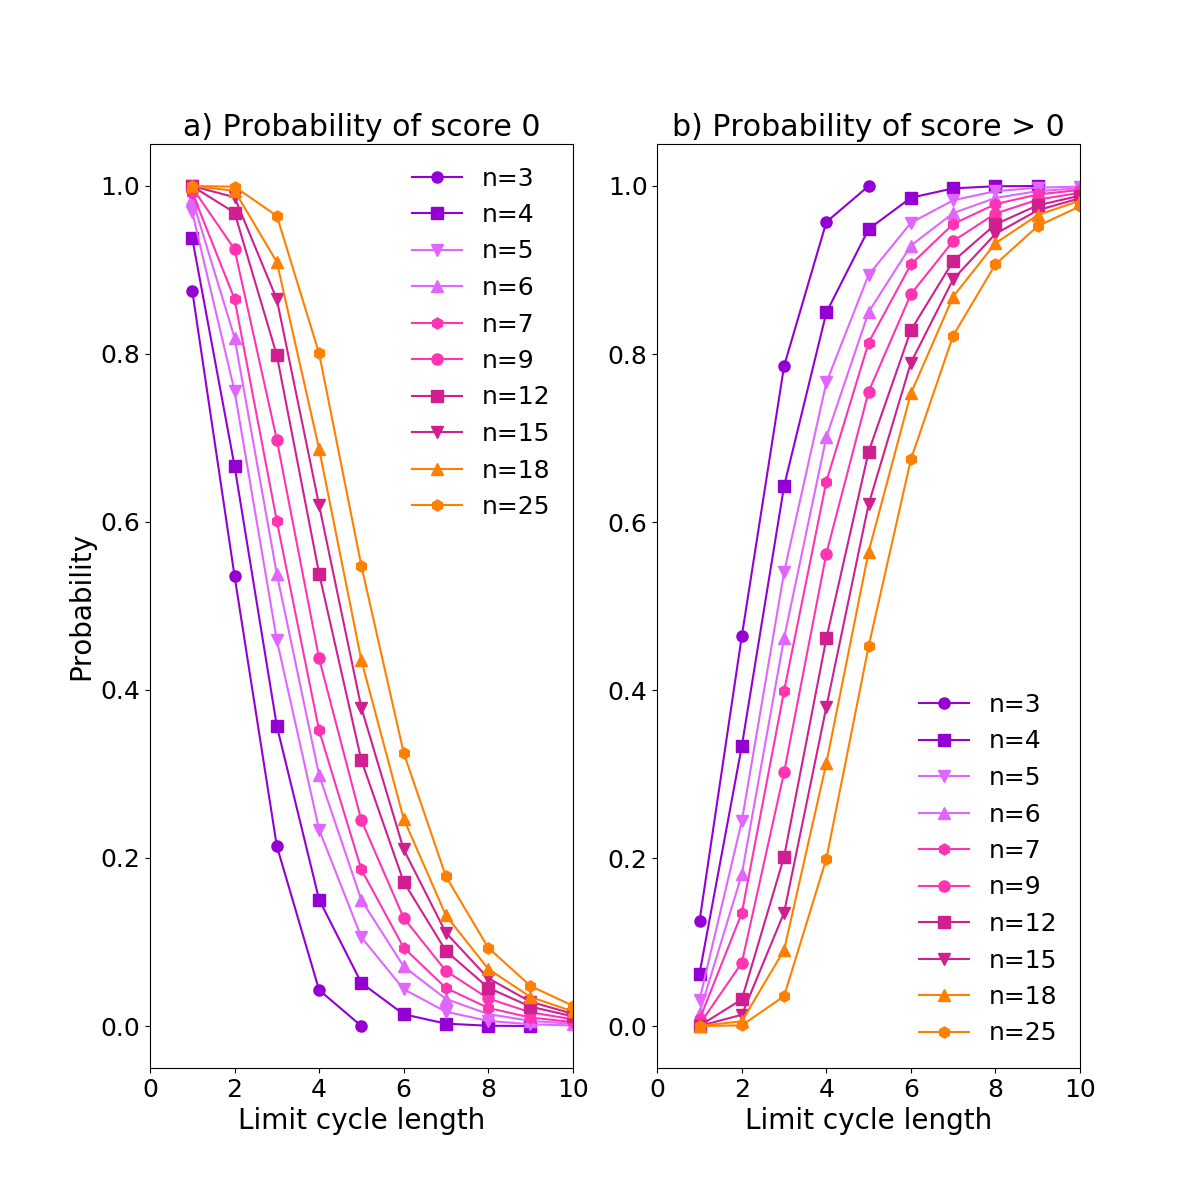
\includegraphics[width=0.9\textwidth,clip=true,trim=0cm 0cm 0cm 0cm]{p0.png}
\caption{\emph{Probability of zero/non-zero score.} The probability of
obtaining a zero or non-zero score for randomly selected limit cycle
state sets of length $l$ in several systems with $3$--$25$ genes.}
\label{fig:p0}
\end{center}
\end{figure}

\section{The genome space}

The genome space is distinct from the gene state space. The genome
space is larger, with $n 2^{n-1}$ bits required to specify the
transitions in a gene space of $n$ genes.

\subsection{Visualising the gene space transitions}

We can plot the gene space transitions in our 5 gene space (Fig.~\ref{fig:genetrans}).

\begin{figure}
\begin{center}
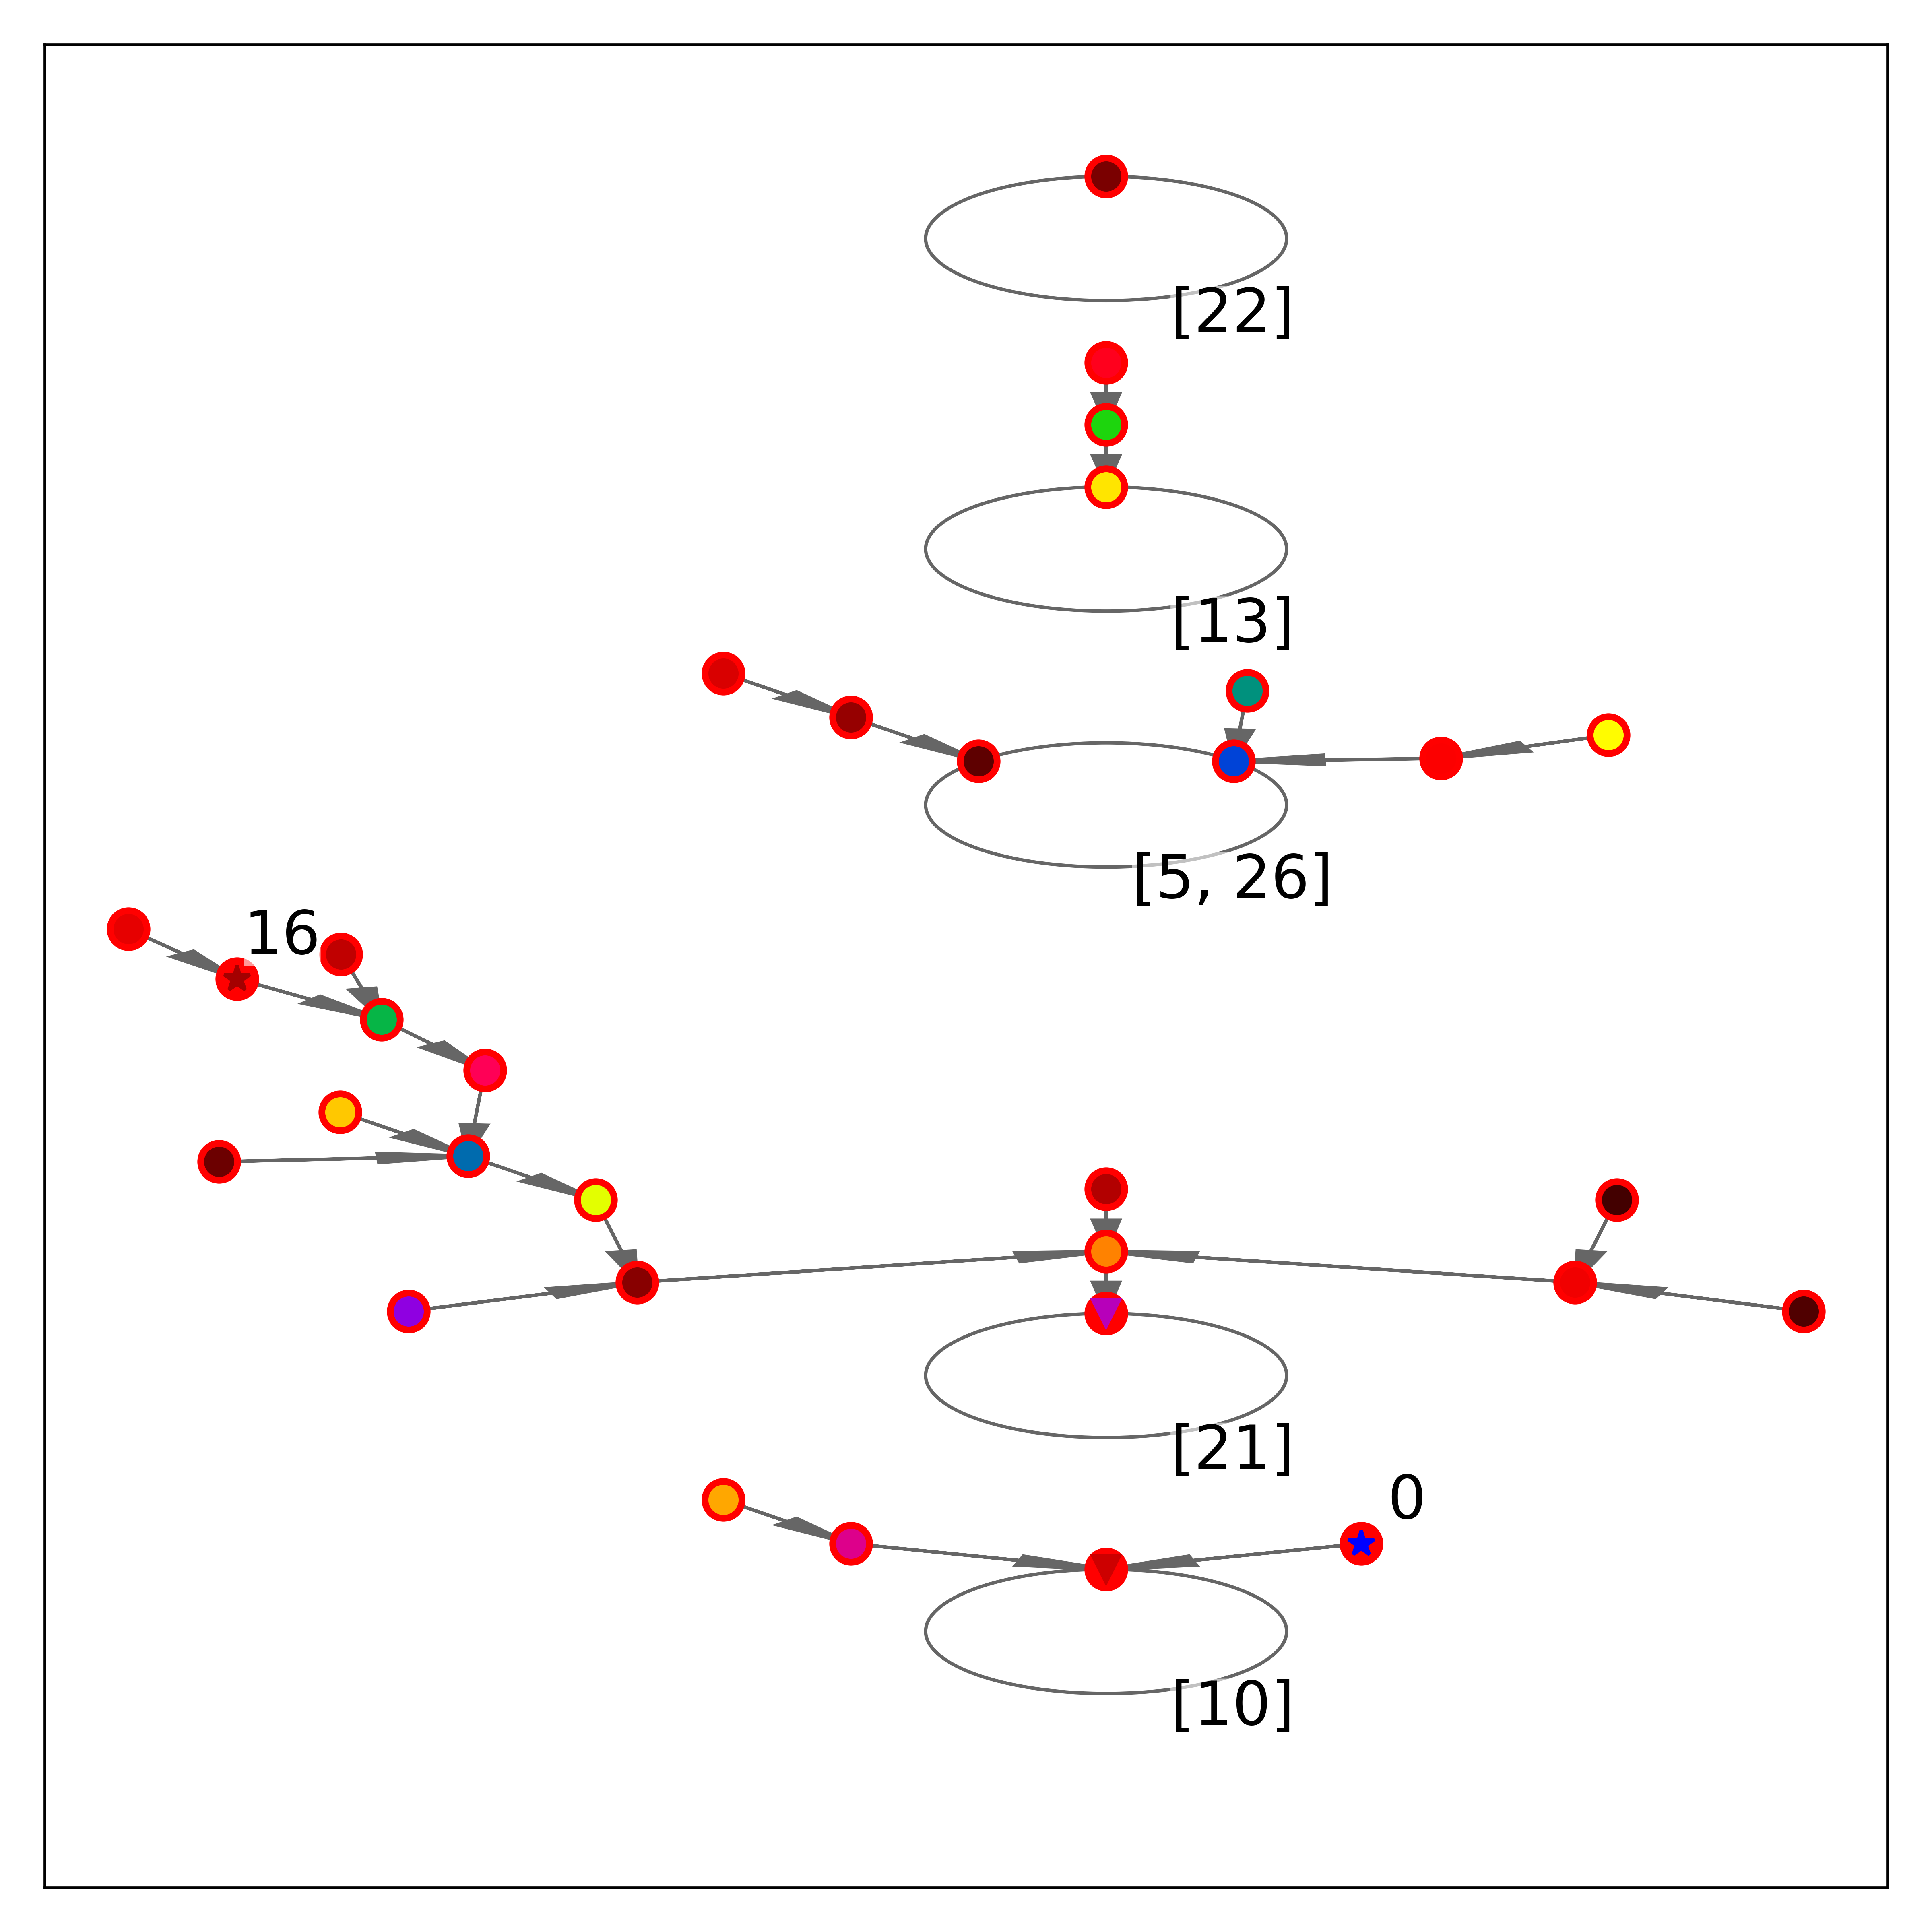
\includegraphics[width=0.6\textwidth,clip=true,trim=0cm 0cm 0cm 0cm]{states_bitflips_flip000.png}
\caption{\emph{Sample gene state transitions.} All $2^5=32$ gene
states in a $5$ gene system. Each state is labelled by colour and by
its value. The states on the limit cycle are labelled in square
brackets. Each state has a transition to a downstream state. Not all
states are transitioned to by another state. The set of all
transitions can be described as a set of pairs of states. For this
network, which is specified by the genome `00011110000010010001000111000110111000100001101101101000011101001010110100011101', that set would include: 15:25, 25:11, 11:09, etc.}
\label{fig:genetrans}
\end{center}
\end{figure}

\subsection{Flipping one bit}

Flipping one bit in the genome space always changes exactly two
transition in the gene state transition diagram (for k=n-1; it's one
for k=n) (Fig.~\ref{fig:genetrans2}). The reason that two states
change for one bit change in the genome, relates to the arrangement of
this gene transition space: only the other $n-1$ inputs determine the
next state of the gene. Consider bit 0 of the genome, which determines
the next state of gene a when the inputs to gene a are [0 0 0
0]. There are two gene states which give this input to gene a: [0 0 0
0 0] and [1 0 0 0 0] and so both of these gene states have their
transition modified when bit 0 of the genome flips.

\begin{figure}
\begin{center}
\includegraphics[width=0.6\textwidth,clip=true,trim=0cm 0cm 0cm 0cm]{states_bitflips_flip02.png}
\caption{\emph{Flip one bit.} The result of flipping bit 2 of the
genome given in Fig.~\ref{fig:genetrans}. Gene state 18 no longer
transitions to gene state 00. Instead, it transitions to gene state
16. Gene state 02 no longer transitions to gene state 04, instead, it
transitions to gene state 20. Two transition changes for one bit
change in the genome.}
\label{fig:genetrans2}
\end{center}
\end{figure}

\subsection{Paths from vertex to vertex}

In the genome space, there are $h!$ `paths' from any genome to another
genome a Hamming distance $h$ away.

The probability of a new genome being fitter, equal or less fit is
shown in Fig.~\ref{fig:prob_fitter}

\begin{figure}
\begin{center}
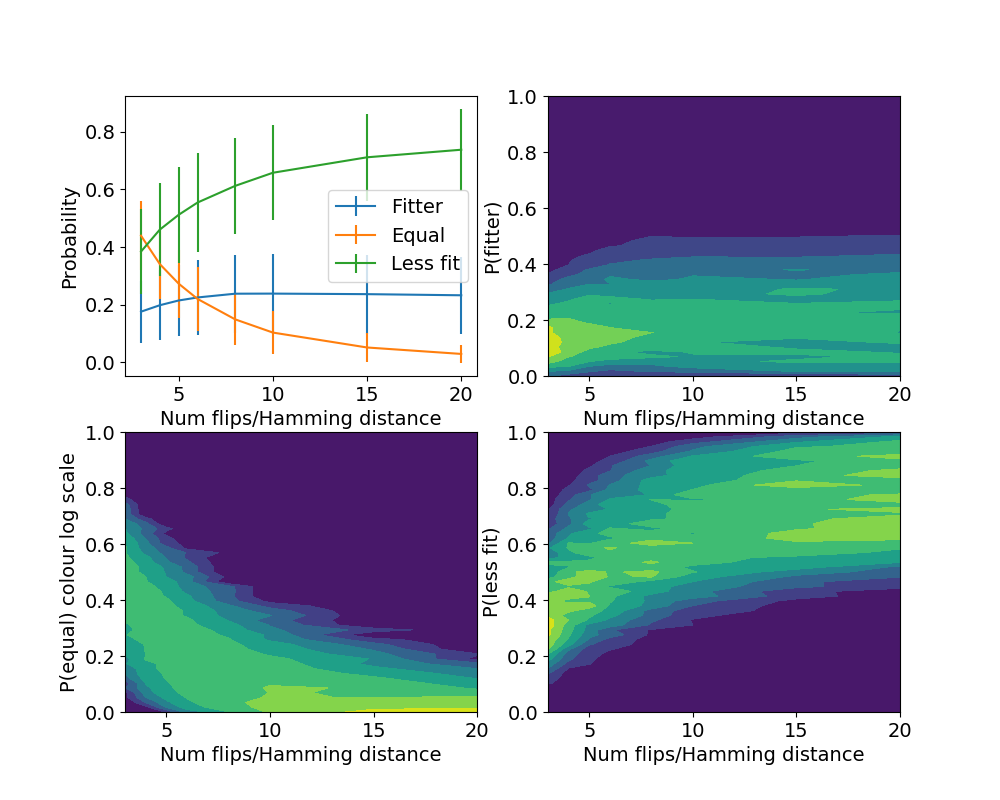
\includegraphics[width=0.7\textwidth,clip=true,trim=0cm 0cm 0cm 0cm]{prob_fitinc_flipbits_prob_vs_bits.png}
\caption{\emph{Probability of finding a fitter state.}
The probability of finding a fitter, equally fit, or less fit state
plotted against the number of bits that are flipped to generate a new
genome. Top left: means, with standard deviations shown as error
bars. For a single bit flip, the probability of finding an equally fit
state is highest. The probability of finding a fitter state is
somewhat independent of the number of bits flipped, with a very wide variance.}
\label{fig:prob_fitter}
\end{center}
\end{figure}


\section{Evolution speed}

% /home/seb/models/Wilson2018EvoGene/simsj/plot/png/evolution_histos_loglog1_nodrift_ff4_fb.png
\begin{figure}
\begin{center}
\includegraphics[width=0.7\textwidth,clip=true,trim=0cm 0cm 0cm 0cm]{evolution_histos_loglog1_nodrift_ff4_fb.png}
\caption{\emph{Evolution rates as function of number of bit flips per
generation.} No drift.}
\label{fig:ev_bf}
\end{center}
\end{figure}

\begin{figure}
\begin{center}
\includegraphics[width=0.7\textwidth,clip=true,trim=0cm 0cm 0cm 0cm]{evolution_histos_loglog1_nodrift_ff4.png}
\caption{\emph{Evolution rates as function of probability of flipping
a big when evolving.} No drift}
\label{fig:ev_prob}
\end{center}
\end{figure}


%
% BIBLIOGRAPHY
%
\selectlanguage{English}
\bibliographystyle{abbrvnotitle}
% The bibliography NoTremor.bib is the one exported from Zotero. It
% may be necessary to run my UTF-8 cleanup script, bbl_utf8_to_latex.sh
%%\bibliography{NoTremor}

%%% Upload the *bib file along with the *tex file and PDF on
%%% submission if the bibliography is not in the main *tex file

\end{document}
